\documentclass{beamer}
% -----PACKAGES
%\usepackage[shortend,titlenumbered]{algorithm2e}
%\usepackage{algorithmic}
%\usepackage[plain]{algorithm}
\usepackage{multicol}
\usepackage{color}
\usepackage{multirow}
\usepackage{fancybox}
%\usepackage{index}
\usepackage{varioref}
\usepackage{psfrag}
\usepackage{epsfig}
\usepackage{boxedminipage}
\usepackage{graphicx}
\usepackage{rotating}
\usepackage{amsmath}
\usepackage{amssymb}
%\usepackage{amsfont}
\usepackage{latexsym}
\usepackage{alltt}
%\usepackage[small,bf]{caption}
\usepackage{url}
%\usepackage{citesort}
%\usepackage{crop}
\usepackage{array}
\usepackage{subfigure}
\usepackage{dcolumn}

% -----SETLENGTH
%\setlength{\captionmargin}{20pt} 

% -----NEWCOMMANDS
\newcommand{\nc}{\newcommand}
\nc{\mathsm}[1]{\text{\small{$#1$}}}
\nc{\ubar}[1]{\underset{-}{#1}}
\nc{\optype}{\textrm}
\nc{\EQ}[1]{(\ref{eq:#1})}
\nc{\TAB}[1]{\ref{tab:#1}}
\nc{\FIG}[1]{\ref{fig:#1}}
\nc{\SEC}[1]{\ref{sec:#1}}
\nc{\ALG}[1]{\ref{alg:#1}}
\nc{\CHAP}[1]{\ref{chap:#1}}
\nc{\mtrx}[1]{\boldsymbol{\mathbf{#1}}}
\nc{\vctr}[1]{\boldsymbol{\mathbf{#1}}}
\nc{\grad}{\mbox{\boldmath$\nabla$}}
\nc{\gradient}{\textsl{grad}\,}
\nc{\hessian}{\textsl{grad\,}^2}
\nc{\ii}{\iota}
\nc{\dd}{d}
\nc{\ee}{\mathrm{e}}
\nc{\pdiv}[2]{\partial{#1}/\partial{#2}}
\nc{\dpdiv}[2]{\displaystyle{\frac{\partial{#1}}{\partial{#2}}}}
\nc{\ddiv}[2]{\displaystyle{\frac{\dd{#1}}{\dd{#2}}}}
\nc{\inpr}{\hspace{-1pt}\cdot\hspace{-1pt}}
\nc{\IR}{\mathbb{R}}
\nc{\IN}{\mathbb{N}}
\nc{\IZ}{\mathbb{Z}}
\nc{\IC}{\mathbb{C}}
\nc{\half}{\frac{1}{2}}
\nc{\shalf}{\scriptstyle{\half}} 
\nc{\ds}[1]{\displaystyle{#1}}
\nc{\ts}[1]{\textstyle{#1}}
\nc{\sign}{\optype{sign}}
\nc{\spr}{\optype{spr}}
\nc{\dist}{\optype{dist}}
\nc{\rank}{\optype{rank}}
\nc{\codim}{\optype{codim}}
\nc{\supp}{\optype{supp}}
\nc{\diag}{\optype{diag}}
\nc{\meas}{\optype{meas}}
\nc{\cond}{\optype{cond}}
\nc{\kernel}{\optype{kernel}}
\nc{\spa}{\optype{span}}
\nc{\order}{\mathcal{O}}
\nc{\Fr}{\mathrm{Fr}}
\nc{\Rey}{\mathrm{Re}}
\nc{\Ord}{O}
\nc{\ord}{o}
\nc{\st}{\:{:}\:}
\nc{\closure}[1]{\overline{#1}}
\nc{\emin}[1]{\emph{#1}\index{#1}\/}
\nc{\rmin}[1]{#1\index{{}@{#1}}}
\nc{\Laplace}{\Delta}
\nc{\ie}{i.e.}
\nc{\eg}{e.g.}
%\nc{\union}{\cup}
\nc{\Union}{\bigcup}
\nc{\lf}[1]{\mathsf{#1}}
\nc{\dbar}[1]{\bar{\bar{#1}}}
\nc{\ul}[1]{\underline{#1}}
\nc{\hpt}{\hspace{0.5pt}}
\nc{\E}[1]{\times{}10^{#1}}
\nc{\inp}[2]{\langle{#1},{#2}\rangle}
\nc{\tmpcommand}{}

% -----RENEWCOMMANDS
\renewcommand{\baselinestretch}{1}
\renewcommand{\exp}{\optype{exp}\,}
\renewcommand{\cosh}{\optype{cosh}\,}
\renewcommand{\tanh}{\optype{tanh}\,}
\renewcommand{\sinh}{\optype{sinh}\,}
\renewcommand{\div}[1]{\optype{div}\,{#1}}
\renewcommand{\half}{\mbox{$\frac{1}{2}$}}
%\renewcommand{\descriptionlabel}[1]{\hspace{\labelsep}\emph{#1}}

% -----ETC
\raggedbottom


\DeclareMathOperator{\curl}{\bf curl}
\DeclareMathOperator{\rot}{\rm curl}
\DeclareMathOperator{\divv}{\rm div}
\newcommand{\tro}{\gamma_0}
\newcommand{\trt}{\gamma_{\sft}}
\newcommand{\trn}{\gamma_{\sfn}}

\newcommand{\PT}{{\partial T}}
\newcommand{\bbN}{{\mathbb{N}}}
\newcommand{\bbP}{{\mathbb{P}}}

\newcommand{\scC}{{\mathscr{C}}}
\newcommand{\caD}{{\mathcal{D}}}
\newcommand{\caL}{{\mathcal{L}}}

\newcommand{\sfe}{{\mathsf{e}}}
\newcommand{\sff}{{\mathsf{f}}}
\newcommand{\sft}{{\boldsymbol{\mathsf{t}}}}
\newcommand{\sfn}{{\boldsymbol{\mathsf{n}}}}

%   Common caligraphic abbrevs
\newcommand{\BB}{\mathcal{B}}
\newcommand{\CC}{\mathcal{C}}
\newcommand{\DD}{\mathcal{D}}
\newcommand{\EE}{\mathcal{E}}
\newcommand{\FF}{\mathcal{F}}
\newcommand{\GG}{\mathcal{G}}
\newcommand{\II}{\mathcal{I}}
\newcommand{\JJ}{\mathcal{J}}
\newcommand{\KK}{\mathcal{K}}
\newcommand{\LL}{\mathcal{L}}
\newcommand{\OO}{\mathcal{O}}
\newcommand{\QQ}{\mathcal{Q}}
\newcommand{\RR}{\mathcal{R}}
\newcommand{\TT}{\mathcal{T}}


 %% JAY'S PREAMBLE
 %%========================

%   Math symbol definitions
\def\d{\partial}
%\newsymbol\lee 132E
\newcommand{\union}{\mathop{\bigcup}}
\newcommand{\intersect}{\mathop{\bigcap}}
\newcommand{\binomial}[2]{\ensuremath{
		\begin{pmatrix}{#1}\\{#2}\end{pmatrix}}}
\newcommand{\smallbinomial}[2]{\ensuremath{
		(\begin{smallmatrix}{#1}\\{#2}\end{smallmatrix})}}
\newcommand{\tang}[1]{\ensuremath{{#1}_{\intercal}}} % can use \top
						     % also
\newcommand{\hypergeom}[2]{\ensuremath{\sideset{_{#1}}{_{#2}}{\mathop{F}}}}
%   Difficult names
\newcommand{\Babuska}{Babu{\v{s}}ka}       % Remember: Usage is \Babuska\
\newcommand{\Cea}{C{\'e}a}                 % with trailing `\' to give space
\newcommand{\Poincare}{Poincar{\'{e}}}     % when needed, but when ending
\newcommand{\Nedelec}{N{\'{e}}d{\'{e}}lec} % sentence use \Babuska.
\newcommand{\Frechet}{Fr{\'{e}}chet}
\newcommand{\Muller}{M{\"u}ller}
\newcommand{\LHospital}{L'H{\^{o}}spital}
%   Bold and beautiful
\newcommand{\ba}{{\boldsymbol{a}}}
\newcommand{\bA}{\boldsymbol{A}}
\newcommand{\balpha}{{\boldsymbol{\alpha}}}
\newcommand{\bB}{{\boldsymbol{B}}}
\newcommand{\bb}{{\boldsymbol{b}}}
\newcommand{\bbeta}{{\boldsymbol{\beta}}}
\newcommand{\etab}{{\boldsymbol{\eta}}}
\newcommand{\bC}{{\boldsymbol{C}}}
\newcommand{\bc}{{\boldsymbol{c}}}
\newcommand{\bD}{{\boldsymbol{D}}}
\newcommand{\bd}{{\boldsymbol{d}}}
\newcommand{\db}{{\boldsymbol{\d}}}
\newcommand{\bdelta}{{\boldsymbol{\delta}}}
\newcommand{\bDelta}{{\boldsymbol{\Delta}}}
\newcommand{\beps}{{\boldsymbol{\varepsilon}}}
\newcommand{\be}{{\boldsymbol{e}}}
\newcommand{\bg}{{\boldsymbol{g}}}
\newcommand{\bm}{{\boldsymbol{m}}}
\newcommand{\bn}{{\boldsymbol{n}}}
\newcommand{\bN}{{\boldsymbol{N}}}
\newcommand{\bp}{{\boldsymbol{p}}}
\newcommand{\bpsi}{{\boldsymbol{\psi}}}
\newcommand{\bq}{{\boldsymbol{q}}}
\newcommand{\bxi}{{\boldsymbol{\xi}}}
\newcommand{\bE}{{\boldsymbol{E}}}
\newcommand{\bF}{{\boldsymbol{F}}}
\newcommand{\bh}{{\boldsymbol{h}}}
\newcommand{\bH}{{\boldsymbol{H}}}
\newcommand{\bI}{{\boldsymbol{I}}}
\newcommand{\bj}{{\boldsymbol{j}}}
\newcommand{\bJ}{{\boldsymbol{J}}}
\newcommand{\bK}{{\boldsymbol{K}}}
\newcommand{\bk}{{\boldsymbol{k}}}
\newcommand{\bll}{{\boldsymbol{\ell}}}
\newcommand{\bL}{{\boldsymbol{L}}}
\newcommand{\blambda}{{\boldsymbol{\lambda}}}
\newcommand{\bmu}{{\boldsymbol{\mu}}}
\newcommand{\bM}{{\boldsymbol{M}}}
\newcommand{\bomega}{{\boldsymbol{\omega}}}
\newcommand{\bP}{{\boldsymbol{P}}}
\newcommand{\bphi}{{\boldsymbol{\phi}}}
\newcommand{\bQ}{{\boldsymbol{Q}}}
\newcommand{\bG}{{\boldsymbol{G}}}
\newcommand{\bu}{{\boldsymbol{u}}}
\newcommand{\bU}{{\boldsymbol{U}}}
\newcommand{\bV}{{\boldsymbol{V}}}
\newcommand{\bX}{{\boldsymbol{X}}}
\newcommand{\bv}{{\boldsymbol{v}}}
\newcommand{\bw}{{\boldsymbol{w}}}
\newcommand{\bW}{{\boldsymbol{W}}}
\newcommand{\bR}{{\boldsymbol{R}}}
\newcommand{\br}{{\boldsymbol{r}}}
\newcommand{\bS}{{\boldsymbol{S}}}
\newcommand{\bT}{{\boldsymbol{T}}}
\newcommand{\btau}{{\boldsymbol{\tau}}}
\newcommand{\bt}{{\boldsymbol{t}}}
\newcommand{\bx}{{\boldsymbol{x}}}
\newcommand{\by}{{\boldsymbol{y}}}
\newcommand{\bz}{{\boldsymbol{z}}}
\newcommand{\bzero}{{\boldsymbol{0}}}
\newcommand{\bZ}{{\boldsymbol{Z}}}
%   Common scalar fields
\newcommand{\RRR}{\mathbb{R}}
\newcommand{\CCC}{\mathbb{C}}
\newcommand{\ZZZ}{\mathbb{Z}}
\newcommand{\NNN}{\mathbb{N}}
%   Differential operators
\newcommand{\dive}{\mathop\mathrm{div}}
%\newcommand{\grad}{\ensuremath{\mathop{{\bf{grad}}}}}
%\newcommand{\curl}{{\ensuremath\mathop{\mathbf{curl}\,}}}
\newcommand{\Curl}{ {\bf Curl}}
\newcommand{\dx}{\ensuremath{\mathrm{d}x}}
\newcommand{\dy}{\ensuremath{\mathrm{d}y}}
\newcommand{\dr}{\ensuremath{\mathrm{d}r}}
\newcommand{\dR}{\ensuremath{\mathrm{d}R}}
\newcommand{\drho}{\ensuremath{\mathrm{d}\rho}}
\newcommand{\dz}{\ensuremath{\mathrm{d}z}}
\newcommand{\dzeta}{\ensuremath{\mathrm{d}\zeta}}
%   Wordy math symbols
\newcommand{\card}{\ensuremath{\mathop\mathrm{card}}}
%\newcommand{\diag}{\ensuremath{\mathop\mathrm{diag}}}
\newcommand{\diam}{\ensuremath{\mathop\mathrm{diam}}}
%\newcommand{\dist}{\mathop\mathrm{dist}}
\newcommand{\Ker}{\mathop\mathrm{Ker}}
\newcommand{\Range}{\mathop\mathrm{Range}}
%\newcommand{\rank}{\mathop\mathrm{rank}}
%\newcommand{\meas}{\mathop\mathrm{meas}}
\newcommand{\Forall}{\quad\text{for all }}
%\newcommand{\supp}{\mathop\mathrm{supp}}
\newcommand{\Span}{\mathop\mathrm{Span}}
\newcommand{\Hdiv}[1]{\bH(\dive,#1)}
%\newcommand{\Hcurl}[1]{\bH(\curl,#1)}
%   Common caligraphic abbrevs
%\newcommand{\BB}{\mathcal{B}}
%\newcommand{\CC}{\mathcal{C}}
%\newcommand{\DD}{\mathcal{D}}
%\newcommand{\EE}{\mathcal{E}}
%\newcommand{\FF}{\mathcal{F}}
%\newcommand{\GG}{\mathcal{G}}
%\newcommand{\II}{\mathcal{I}}
%\newcommand{\JJ}{\mathcal{J}}
%\newcommand{\KK}{\mathcal{K}}
%\newcommand{\LL}{\mathcal{L}}
%\newcommand{\OO}{\mathcal{O}}
%\newcommand{\QQ}{\mathcal{Q}}
%\newcommand{\RR}{\mathcal{R}}
%\newcommand{\TT}{\mathcal{T}}
%   Variations on standard symbols
\newcommand{\veps}{\varepsilon}
\newcommand{\vlam}{\varLambda}
\newcommand{\vpi}{\varPi}
\newcommand{\vPi}{\boldsymbol{\varPi}}
\newcommand{\vsig}{\varSigma}
\newcommand{\vbt}{\boldsymbol{\varTheta}}
\newcommand{\vPsi}{\boldsymbol{\varPsi}}
%\newcommand{\ii}{\hat{\imath}}
%   Innerproducts, norms, etc
\newcommand{\ntrip}[1]{|\!|\!| {#1} |\!|\!|}
\newcommand{\ip}[1]{\langle {#1} \rangle}
%   Utilities
\newcommand{\blnk}{\underline{\hspace{3cm}}\;}
\newcommand{\marg}[1]{\marginpar{\tiny{\framebox{\parbox{1.7cm}{#1}}}}}
\newcommand{\degreeC}[1]{\ensuremath{{#1\,}^\circ\!\text{C}}}
                        % try also  \textcelsius of textcomp package
%   Trademarked names \texttrademark, \textregistered
\newcommand{\matlab}{MATLAB\textregistered\renewcommand{\matlab}{MATLAB}}
\newcommand{\femlab}{FEMLAB\textregistered\renewcommand{\femlab}{FEMLAB}}

%   Style preferences
\renewcommand{\thefootnote}{\fnsymbol{footnote}} % Use symbols instead of
						 % numbers for footnotes
						 

\newcommand{\Eg}{\EE^\mathrm{grad}}
\newcommand{\Ec}{\boldsymbol{\EE}^\mathrm{curl}}
\newcommand{\Ed}{\boldsymbol{\EE}^\mathrm{div}}


\newcommand{\bfdu}{\mbox{\boldmath $\delta u$}}
\newcommand{\bfdv}{\mbox{\boldmath $\delta v$}}
\newcommand{\du}{{\delta u}}
\newcommand{\dv}{{\delta v}}
\newcommand{\bfnabt}{\widetilde{\bfnab}}
\newcommand{\bfepst}{\widetilde{\bfeps}}

\usetheme[secheader]{pecostalk}
\usepackage{comment}
% \usepackage{subfig}
\graphicspath{{figs/}}

\newcommand{\pecosbold}[1]{{\color{pecos2}{#1}}}
\newcommand{\pecosreallybold}[1]{{\color{pecos6}{#1}}}

\author[Truman. E. Ellis]{Truman E. Ellis}
\title[Locally Conservative DPG]{Locally Conservative Discontinuous
Petrov-Galerkin for Fluid Problems}
\institute{Institute for Computational and Engineering Sciences\\
The University of Texas at Austin}
\date{July 25, 2013}

\begin{document}

\begin{frame}
\begin{center}

\includegraphics[width=.8\linewidth]{grand_logo}\\
\end{center}
\titlepage
\end{frame}
\begin{comment}
My name is Truman Ellis, and I am also working in Dr. Demkowicz's group on the
discontinuous Petrov-Galerkin method. My background is in aerospace
engineering and CFD, and my goal is to help develop DPG into an attractive
method for realistic problems in computational fluid dynamics. So the goal is
to work on the Euler equations and then build on Nate and Jesse's work on
laminar Navier-Stokes with some turbulence modeling.  But before I got into
that, we thought it would be useful to study a topic that keeps coming up from
the CFD community. Is DPG locally conservative?

This is a numerical characteristic close to the heart of many CFD
practitioners, and in order for DPG to gain a certain level of acceptance
among these circles, we need to address some of these concerns. There are also
some mathematically attractive reasons to pursue local conservation. The
Lax-Wendroff theorem guarantees that a convergent numerical solution to a
system of hyperbolic conservation laws will converge to the correct weak
solution. Also, we are focusing on local conservation on the
convection-diffusion equation as a proof of concept. We are working on
extending this work to more realistic flow simulations.
\end{comment}


%===============================================================================
% NEW SLIDE
%===============================================================================
\begin{frame}
\frametitle{A Summary of DPG}
Overview of Features
\begin{itemize}
\item Robust for singularly perturbed problems
\item Stable in the preasymptotic regime
\item Designed for adaptive mesh refinement
\end{itemize}
\bigskip

DPG is a minimum residual method:
\[
u_{h} = \underset{w_{h} \in U_{h}} \argmin \,\, \frac{1}{2}
\norm{Bw_{h}-l}_{V'}^{2}
\]
\vspace{-1em}
\[
\scalebox{1.8}{\ensuremath{\Updownarrow}}
\]
\vspace{-1em}
\[
b(u_h,R_V^{-1}B\delta u_h)
=l(R_V^{-1}B\delta u_h)
\quad\forall\delta u_h\in U_h
\]
where $v_{\delta u_h}:=R_V^{-1}B\delta u_h$ are the
\pecosbold{optimal test functions}.
\end{frame}
\begin{comment}
For the sake of avoiding a lot of repetition and making sure we all finish on
time, I'm going to offer an extremely condensed summary of DPG. Nate and Jesse
already covered this stuff with more rigor. So what are DPG's main selling
points? Why are we interested in applying it to complicated fluid problems
(eventually).
For one, DPG has proven very robust in the face of singularly
perturbed problems which holds promise for high Reynolds number flows.
You do not need a domain expert to craft well designed meshes for each new
problem. We are mathematically guaranteed to remain stable under very coarse
meshes while adaptively refining toward a solution.

And mathematically, how can we classify DPG? By derivations, it is a minimum
residual method. This means that through the choice of specific optimal test
functions we automatically minimize the residual in the dual norm of a
Hilbert space V. We also have a well-defined process to generate the optimal
test functions which is computationally feasible.
\end{comment}


%===============================================================================
% NEW SLIDE
%===============================================================================
\begin{frame}
\frametitle{DPG for Convection-Diffusion}
Start with the strong-form PDE.
\[
\nabla\cdot(\bfbeta u)-\epsilon\Delta u = g
\]
Rewrite as a system of first-order equations.
\begin{align*}
\nabla\cdot(\bfbeta u-\bfsigma)&=g\\
\frac{1}{\epsilon}\bfsigma-\nabla u&=\boldsymbol0
\end{align*}
Multiply by test functions and integrate by parts over each element, $K$.
\begin{align*}
-(\bfbeta u-\bfsigma,\nabla v)_K+((\bfbeta
u-\bfsigma)\cdot\mathbf{n},v)_{\partial K}&=(g,v)_K\\
\frac{1}{\epsilon}(\bfsigma,\bftau)_K+(u,\nabla\cdot\bftau)_K
-(u,\tau_n)_{\partial K}&=0
\end{align*}
Use the ultraweak (DPG) formulation to obtain bilinear form $b(u,v)=l(v)$.
\begin{align*}
-(\bfbeta u-\bfsigma,\nabla v)_K&+(\hat f,v)_{\partial K}
+ \frac{1}{\epsilon}(\bfsigma,\bftau)_K\\
&+(u,\nabla\cdot\bftau)_K
-(\hat u,\tau_n)_{\partial K}=(g,v)_K
\end{align*}
\end{frame}
\begin{comment}
With that ultra-brief refresher, we can now apply DPG to the
convection-diffusion equation. We prefer to work with systems of first order
equations. Then, multiplying the top equation by a scalar valued test
function, v, and the second by a vector valued test function tau, we can
integrate by parts over each element, K. Combining the two equations, we get
our bilinear form for convection diffusion. We seek the field variable, u and
sigma in L2, but that leaves their traces undefined. So, in a manner similar
to the hybridized DG method, we define new unknowns for our traces and fluxes,
u hat and f hat.
\end{comment}


%===============================================================================
% NEW SLIDE
%===============================================================================
\begin{frame}
\frametitle{Local Conservation}
The local conservation law in convection diffusion is
\[
\int_{\partial K}\hat f=\int_K g\,,
\]
which is equivalent to having $\mathbf{v}_K:=\{v,\bftau\}=\{1_K,\boldsymbol0\}$ in the test space.
In general, this is not satisfied by the optimal test functions.
Following Moro et al\textsuperscript{\cite{MoroNguyenPeraire11}} (also
Chang and Nelson\textsuperscript{\cite{ChangNelson1997}}), we
can enforce this condition with Lagrange multipliers:
\begin{align*}
L(u_h,\bflambda) = \frac{1}{2}\norm{R_V^{-1}(Bu_h-l)}_V^2
-\sum_K\lambda_K\underbrace{\langle Bu_h-l,\mathbf{v}_K\rangle}_
{\langle\hat f, 1_K\rangle_{\partial K}-\langle g,1_K\rangle_K}\,,
\end{align*}
where $\bflambda=\{\lambda_1,\cdots,\lambda_N\}$.
\end{frame}
\begin{comment}
So what does local conservation mean for the convection-diffusion equation. We
want the integral of our fluxes over the element faces to be balanced by any
source terms in the RHS. This is equivalent to having one in the test space.
You can see this if you look at the bilinear form on the previous slide and
plug one and zero in as test functions. Unfortunately the optimal test
functions do not always span constants. It turns out we can augment our test
space with constants through the use of Lagrange multipliers. So taking a
couple of steps backward in the abstract form, we can augment our system with
the Lagrange multipliers enforcing local conservation.
\end{comment}


%===============================================================================
% NEW SLIDE
%===============================================================================
\begin{frame}
\frametitle{Local Conservation}
Finding the critical points of $L(u,\bflambda)$, we get the following
equations\textsuperscript{\cite{EllisDemkowiczChan2013}}.
\begin{align*}
\frac{\partial L(u_h,\bflambda)}{\partial u_h}&=b(u_h,R_V^{-1}B\delta u_h)
-l(R_V^{-1}B\delta u_h)\\
&{\color{red}-\sum_K\lambda_K b(\delta
u_h,\mathbf{v}_K)}=0\quad\forall\delta u_h\in U_h
\end{align*}
\[
\frac{\partial
L(u_h,\bflambda)}{\partial\lambda_K}=-b(u_h,\mathbf{v}_K)+l(\mathbf{v}_K)=0\quad\forall
K
\]
A few consequences:
\begin{itemize}
\item We've turned our minimization problem into a saddlepoint problem.
% \item New $\lambda_K$ DOFs can be statically condensed out.
\item Only need to find the optimal test function in the orthogonal complement
of constants. % Backup slide
\end{itemize}
\end{frame}
\begin{comment}
Now, proceeding forward again and setting the derivatives to zero, we have
turned our minimization problem into a saddle point problem. Note that we have
added extra DOFs equal to the number of mesh elements, but the structure of
the problem allows these to be statically condensed out. The most interesting
consequence of this modification (apart from enforcing local conservation) is
that we can modify the search space for our optimal test functions to be
the orthogonal complement of constants.
\end{comment}


%===============================================================================
% NEW SLIDE
%===============================================================================
\begin{frame}
\frametitle{Optimal Test Functions}
For each $\mathbf{u}=\{u,\bfsigma,\hat u,\hat f\}\in\mathbf{U}_h$, find
$\mathbf{v}_{\mathbf{u}}=\{v_\mathbf{u},\bftau_\mathbf{u}\}\in\mathbf{V}$ such that
\[
(\mathbf{v_u},\mathbf{w})_\mathbf{V}=b(\mathbf{u},\mathbf{w})\quad\forall\mathbf{w}\in\mathbf{V}
\]
where $\mathbf{V}$ becomes $\mathbf{V}_{p+\Delta p}$ in order to make this
computationally tractable.

We recently developed this modification to the \emph{robust test norm}
\textsuperscript{\cite{ChanHeuerThanhDemkowicz2012}} which behaves better in
the presence of singularities.
\begin{minipage}[t][1.5in]{\textwidth}
\begin{align*}
\norm{(v,\bftau)}^2_{\mathbf{V},\Omega_h}&=
\norm{\min\left\{\frac{1}{\sqrt{\epsilon}},\frac{1}{\sqrt{|K|}}\right\}\bftau}^2
+\norm{\nabla\cdot\bftau-\bfbeta\cdot\nabla v}^2\\
&+\norm{\bfbeta\cdot\nabla v}^2+\epsilon\norm{\nabla v}^2
\underbrace{\color{red}{
\begin{minipage}[c][0.3in][c]{0.9in}$
\only<1>{
\hspace{1.5ex}
+\norm{v}^2
}
\only<2>{
+\left(\frac{1}{|K|}\int_Kv\right)^2
}$
\end{minipage}
}}_{\only<1>{\text{No longer necessary}}\only<2>{\text{Zero mean term}}}
\end{align*}
\end{minipage}
\end{frame}
\begin{comment}
So how does this affect our search for optimal test functions? The process to
compute optimal test functions is as follows. For each trial function we are
considering, we want to find the test function in an enriched space that
satisfies the following relation - that the inner product of vu with w equals
the bilinear form acting on u and w for all w in V.

The choice of norm on V can significantly affect the robustness of the
solution. Unfortunately, the optimal test norm is not localizable, and for
convection diffusion, the quasi-optimal test norm has boundary layers arising
from the adjoint and thus has approximability issues. Fortunately a
couple of collaborators developed a robust test norm for convection-diffusion.
Sadly, this norm also has its issues as the final zero order term in the
expression is somewhat troublesome. (???)

Why can we replace the L2 term with the zero mean term?
Why is zero mean more friendly than L2?
- Not mesh dependent
- No boundary layers
\end{comment}


%===============================================================================
% NEW SLIDE
%===============================================================================
\begin{frame}
\frametitle{Stability Analysis}
We follow Brezzi's theory for an abstract mixed problem:
\begin{equation*}
\left\{
\begin{array}{lll}
\bfu \in \bfU, p \in Q\\
a(\bfu,\bfw) + c(p,\bfw) & = l(\bfw) & \forall \bfw \in \bfU \\
c(q,\bfu) & = g(q) & \forall q \in Q
\end{array}
\right.
\end{equation*}
where $a,c,l,g$ denote the appropriate
bilinear and linear forms. Note that $a(\bfu,\bfw)=b(\bfu,T\bfw)=(T\bfu,T\bfw)_V$.

Let $\bfpsi$ denote the $\bfH(\text{div},\Omega)$ extension of flux $\hat{f}$
that realizes the minimum in the definition of the quotient (minimum energy
extension) norm.

The norm for the Lagrange multipliers $\lambda_K$ is implied
by the quotient norm used for $H^{-1/2}(\Gamma_h)$ and continuity
bound for form $c(p,\bfw)$:
\[
||\bflambda||:=\left(\sum_K \mu(K) \lambda_K^2\right)^{1/2}
\]
\end{frame}
\begin{comment}
In the following analysis, we neglect the error due to the approximation of optimal test functions.

We skip some of the math needed to show this, but it is pretty trivial. The
full details will be in the ICES report.
\end{comment}


%===============================================================================
% NEW SLIDE
%===============================================================================
\begin{frame}
\frametitle{Inf Sup Condition}
\only<1>{
The inf-sup condition relating spaces $\bfU$ and $Q$ is
\[
\sup_{\bfw \in \bfU} \frac{| c(p,\bfw) |}{|| \bfw ||_{\bfU}} \geq \beta ||
p ||_Q
\]
Let
\begin{equation*}
R\, : \, L^2(\Omega) \ni q \to \bfpsi \in \bfH(\text{div},\Omega) \cap \bfH^1(\Omega)
=\bfH^1(\Omega)
\end{equation*}
be
the continuous right inverse of the divergence operator constructed by
Costabel and McIntosh\textsuperscript{\cite{CostabelMcIntosh}}.
Let $\bfpsi_h$ denote the classical, lowest order Raviart-Thomas (RT) interpolant of
function
\begin{equation*}
\bfpsi = R (\sum_K \lambda_K 1_K)
\end{equation*}
Note that $\text{div} \bfpsi_h = \text{div} \bfpsi = \lambda_K$ in element $K$.
}
\only<2>{
Classical $h$-interpolation interpolation error estimate for the lowest error
Raviart-Thomas elements and continuity of operator $R$ imply the stability estimate:
\begin{equation*}
\begin{array}{lll}
|| \bfpsi_h || & \leq || \bfpsi_h - \bfpsi || + || \bfpsi ||\\[8pt]
&\leq C h || \bfpsi ||_{H^1} +  || \bfpsi || \\[8pt]
& \leq C || \text{div} \bfpsi || = C (\sum_K \mu(K) \lambda_K^2)^{1/2}
\end{array}
\end{equation*}
Let $\hat{f}$ be the trace of $\bfpsi_h$, then
\begin{align*}
\sup_{\hat{f} \in H^{-1/2}(\Gamma_h)} \frac{|  \sum_K \lambda_K \langle
\hat{f},1_K \rangle_{\partial K} |}{|| \hat{f} ||_{H^{-1/2}(\Gamma_h)}}
&\geq \frac{| \sum_K \lambda_K \int_K \text{div} \bfpsi_h \: 1_K  |}
{|| \bfpsi_h ||_{H(\text{div},\Omega)}}\\
&\geq \frac{1}{C} (\sum_K \mu(K) \lambda_K^2)^{1/2}
\end{align*}
}
\end{frame}
\begin{comment}
We proceed now with the discussion of the discrete inf-sup stability
constants. We skip index h in the notation.

Note that C is a generic, mesh independent constant incorporating the constant
from the interpolation error estimate and the continuity constant of R.

Notice that we have considered traces of lowest order Raviart-Thomas elements
for the discretization of the flux.

The inf-sup condition for the lowest order RT spaces implies automatically the
analogous condition for elements of arbitrary order; increasing space U only
makes the discrete inf-sup constant bigger.
\end{comment}


%===============================================================================
% NEW SLIDE
%===============================================================================
\begin{frame}
\frametitle{Inf Sup in Kernel Condition}
We characterize the ``kernel'' space:
\begin{equation*}
\begin{array}{rl}
\bfU_0  := & \{ \bfw \in \bfU \, : \, c(q,\bfw) = 0 \quad \forall q \in Q\} \\[8pt]
 = &\{ (u,\bfsigma,\hat{u},\hat{t}) \, : \, \langle \hat{t},1_K \rangle = 0
 \quad \forall K \}
\end{array}
\end{equation*}
With $\bfu \in \bfU_0$, we have then:
\begin{align*}
   \sup_{\bfw \in \bfU_0} \frac{| a(\bfu,\bfw) |}{|| \bfw ||_{\bfU} }
   &\geq \frac{| b(\bfu,T \bfu) |}{|| \bfu ||}
   = \frac{| b(\bfu,T \bfu) |}{|| T\bfu ||}\frac{||T\bfu||}{||\bfu||}\\
   &= \sup_{(v,\bftau)}\frac{| b((u,\bfsigma,\hat{u},\hat{t}), (v,\bftau)) |}{|| (v,\bftau) ||}
   \frac{||T\bfu||}{||\bfu||}
   \geq \gamma^2 || (u,\bfsigma,\hat{u},\hat{t}) ||
\end{align*}
where $\gamma$ is the stability constant for the standard continuous DPG formulation.

The FE error is bounded by the best approximation error. Note that the exact
Lagrange multipliers are zero, so the best approximation error involves only
the solution $(u,\bfsigma,\hat{u},\hat{t})$.
\end{frame}
\begin{comment}
This is satisfied automatically due to the use of optimal test functions.

In other words, the kernel space contains only the equilibrated fluxes.

The first inequality follows as we plug in the definition for a and pick w=u.
The second equality is trivial, while the next one follows by definition of
the optimal test functions given through the trial-to-test operator T .
\end{comment}


%===============================================================================
% NEW SLIDE
%===============================================================================
\begin{frame}
\frametitle{Robustness Analysis}
\begin{itemize}
  \item We prove robustness of the restricted DPG method by switching to the
    energy norm in Brezzi's stability analysis.
  \item The inf-sup in kernel condition is simple. Upon replacing the original
    norm of solution $\bfu$ with the energy norm, $\gamma$ and the continuity
    constant become one.
  \item In order to investigate the robustness of inf-sup constant $\beta$, we
    need to understand what the energy norm of flux variable $\hat f$ is.
  \item For an element, $K$, we solve for the optimal test functions,
    $v_K\in H^1(K)$, and $\bftau_K\in\bfH(\text{div},K)$
    corresponding to flux $\hat f$:
    \[
    ( (v_K,\bftau_K),(\delta v,\delta\bftau) )_V=\LRa{\hat f,\delta v}
    \quad\forall\delta v\in H^1(K),\,\delta\bftau\in\bfH(\text{div},K)
    \]
  \item The energy norm for $\hat f$ is then
    \[
    ||\hat f||_E^2=\sum_K||(v_K,\bftau_K)||_V^2
    \]
\end{itemize}
\end{frame}
\begin{comment}
  With robust test norms, standard DPG delivers a robust error bound because
  it minimizes the residual in the energy norm. Restricted DPG no longer
  minimizes the residual, so can we claim robustness for this version as well?
\end{comment}


%===============================================================================
% NEW SLIDE
%===============================================================================
\begin{frame}
\frametitle{Robustness Analysis}
\begin{itemize}
    \item Need to establish conditions under which the inf-sup constant is
      independent of viscosity.
      \begin{equation*}
        \sup_{\hat{f}} \frac{| \sum_K \lambda_K \langle \hat{f},1_K \rangle |}{|| \hat{f} ||_E}
        \geq  \beta \LRp{\sum_K \mu(K) \lambda_K^2}^{1/2}
      \end{equation*}
    \item Select $\hat f$ as the trace of the Raviart-Thomas interpolant
      $\bfpsi_h$ of $\bfpsi=R(\sum_K\lambda_K1_K)$.
    \item Proceed as in the previous analysis, but evaluation of the norm of
      $\hat f$ requires a local solve.
      \begin{align*}
        ( (v,\bftau),&(\delta v,\delta\bftau) )_V
        =\LRa{\hat f,\delta v}_{\partial K}
        =\int_K\text{div}\bfpsi_h\delta v
        =\int_K\text{div}\bfpsi\delta v\\
        &=\int_K\lambda_K\delta v=\lambda_K(1_K,\delta v)_K
        \quad\forall\delta v\in
        H^1(K)\,\forall\delta\bftau\in\bfH(\text{div},K)
      \end{align*}
\end{itemize}
\end{frame}
\begin{comment}
We need to establish sufficient conditions under which the inf-sup and continuity constants for the bilinear
form representing the constraint are independent of viscosity

R is the right inverse of the divergence operator constructed by Costabel and
McIntosh.
\end{comment}


%===============================================================================
% NEW SLIDE
%===============================================================================
\begin{frame}
\frametitle{Robustness Analysis}
\begin{itemize}
    \item We need an upper bound for the energy norm of $(v_h,\bftau_h)$:
      \[
      \LRp{\sum_K||(v,\bftau)||^2_V}^{1/2}
      \]
    \item Substituting $(v,\bftau)$ for $(\delta v,\delta\bftau)$ in the
      previous slide:
      \[
      ||(v,\bftau)||^2_V=\lambda_K(1_K,v_k)
      \]
    \item With a robust stability estimate
      $
      (1_K,v_K)\leq C\mu(K)^{1/2}||(v,\bftau)||_K\,,
      $
      \[
      ||(v,\bftau)||_V\leq C\mu(K)^{1/2}|\lambda_K|
      \]
      \[
      \sum_K||(v,\bftau)||_V^2\leq C^2\sum_K\mu(K)\lambda_K^2
      \]
      which leads to the robust estimate of inf-sup constant $\beta$.
\end{itemize}
\end{frame}
\begin{comment}
\end{comment}


%===============================================================================
% NEW SLIDE
%===============================================================================
\begin{frame}
\frametitle{Robustness Analysis}
\begin{itemize}
    \item Finally, we need a continuity estimate on
      \[
      \sum_K\lambda_K\langle\hat f,1_K\rangle
      \]
    \item Testing with $(1_K,\boldsymbol0)$ in the local problem, we obtain
      \[
      ( (v,\bftau),(1_K,\boldsymbol0) )_V=\langle\hat f,1_K\rangle_{\partial K}
      \]
    \item With a robust estimate $|( (v,\bftau),(1_K,\boldsymbol0) )_V|\leq
      C\mu(K)^{1/2}||(v,\bftau)||_V$,
      \begin{align*}
        |\sum_K\lambda_K\langle\hat f,1_K\rangle|
        &\leq C\LRp{\sum_K\mu(K)\lambda_K^2}^{1/2}\LRp{\sum_K||(v,\bftau)||_V^2}^{1/2}\\
        &=C\LRp{\sum_K\mu(K)\lambda_K^2}^{1/2}||\hat f||_E
      \end{align*}
\end{itemize}
\end{frame}
\begin{comment}
With the robust stability and continuity constants for the mixed problem, the
energy error of solution and Lagrange multipliers is bounded robustly by the
best approximation error measured in the energy norm. We arrive thus at the
same situation as in standard DPG.
\end{comment}


%===============================================================================
% NEW SLIDE
%===============================================================================
\begin{frame}
\frametitle{Erickson-Johnson Problem}
On domain $\Omega=[0,1]^2$, with $\beta=(1,0)^T$, $f=0$ and boundary
conditions
\[
\hat f=u_0,\quad\beta_n\le0\,,\quad\quad\hat u=0,\quad\beta_n > 0
\]
Separation of variabes gives an analytic solution
\[
u(x,y)=C_0+\sum_{n=1}^\infty C_n
\frac{\exp(r_2(x-1))-\exp(r_1(x-1))}{r_1\exp(-r_2)-r_2\exp(-r_1)}
\cos(n\pi y)
\]
\vspace{-5ex}
\begin{columns}[b]
\begin{column}{0.5\textwidth}
\begin{figure}[t]
\centering
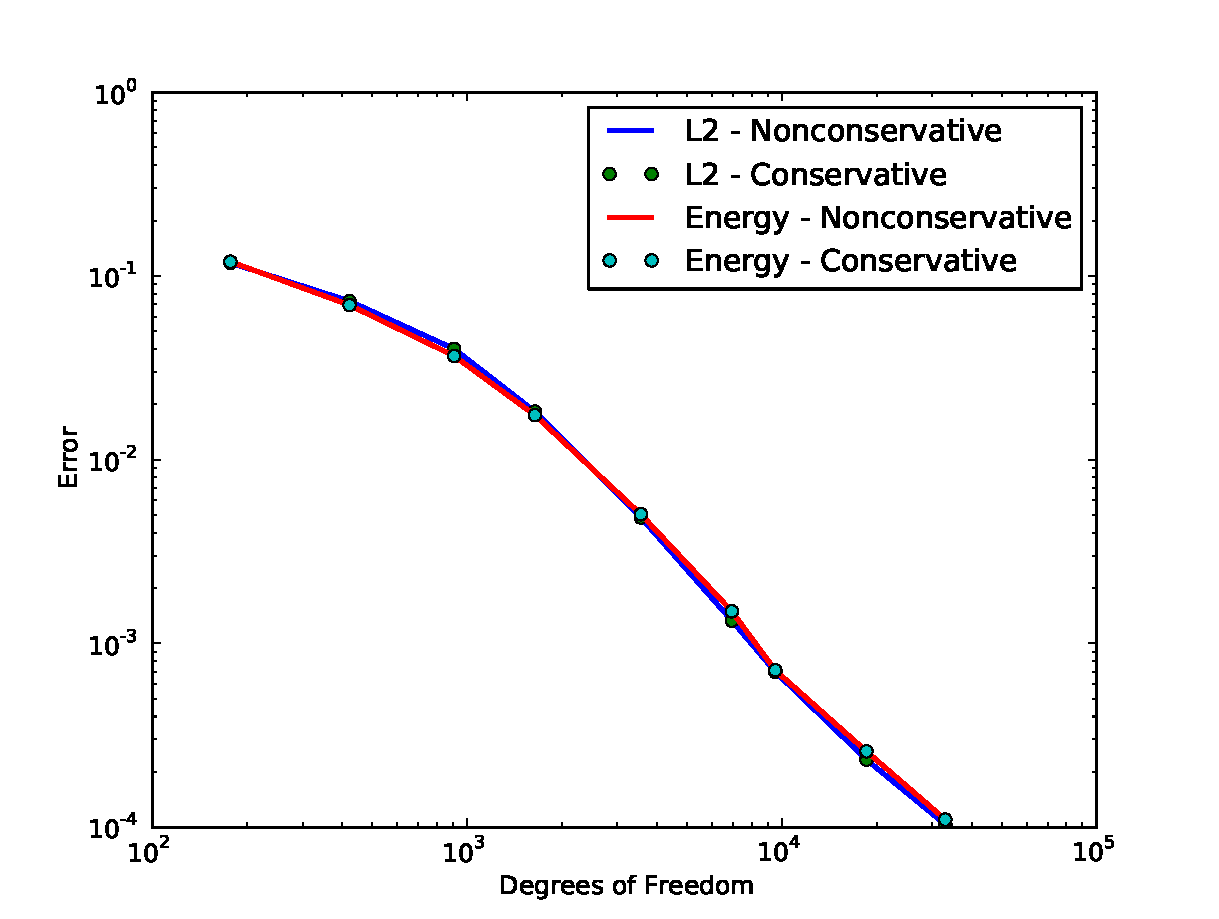
\includegraphics[width=0.9\textwidth]{Erickson/modifiedError.pdf}

\end{figure}
\end{column}
\begin{column}{0.5\textwidth}
\begin{figure}[t]
\centering
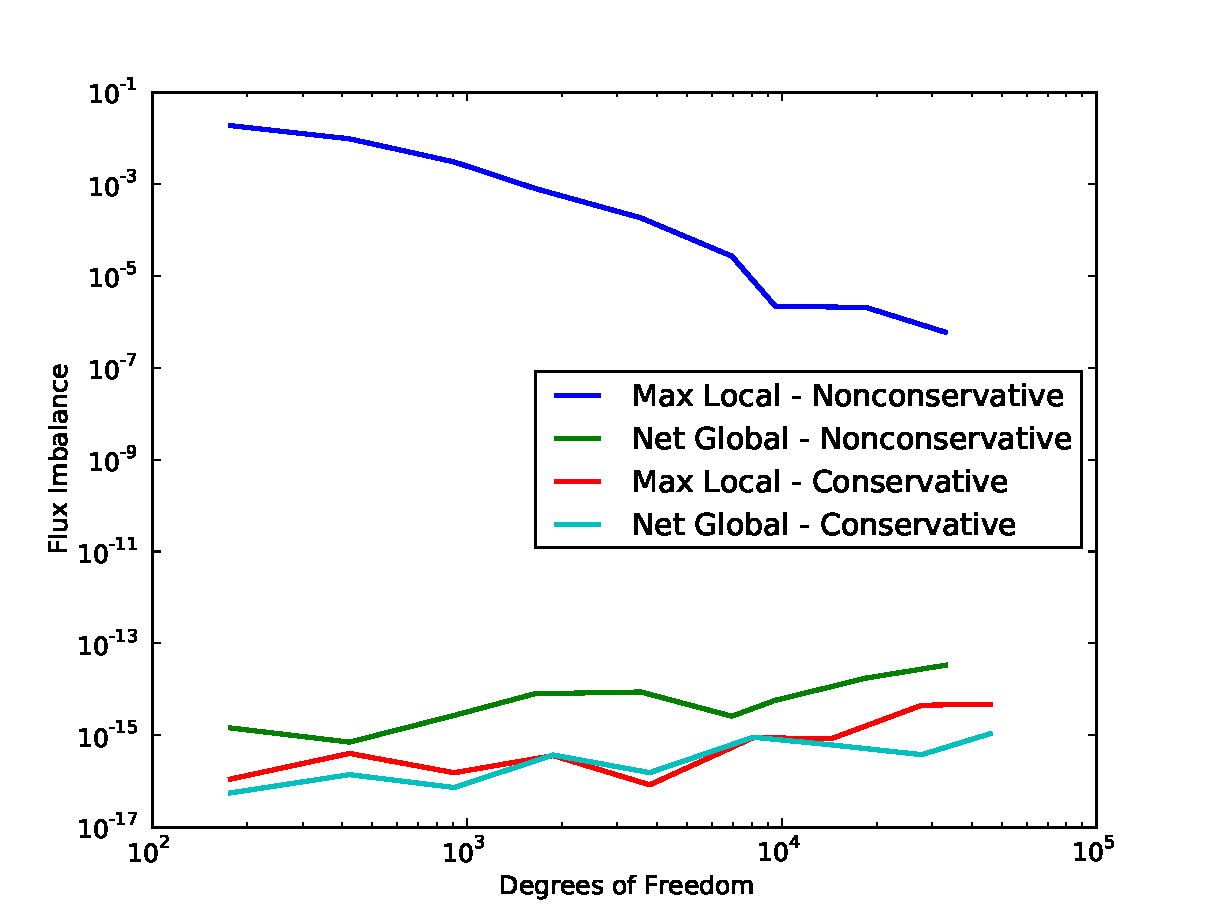
\includegraphics[width=0.9\textwidth]{Erickson/modifiedFlux.pdf}

\end{figure}
\end{column}
\end{columns}
\end{frame}
\begin{comment}
\end{comment}


%===============================================================================
% NEW SLIDE
%===============================================================================
\begin{frame}
\frametitle{Vortex Problem}
After 6 refinements, $\epsilon=10^{-4}$, $\bfbeta=(-y,x)^T$
\only<1>{
\begin{columns}
\begin{column}{0.49\textwidth}
\begin{figure}
\centering
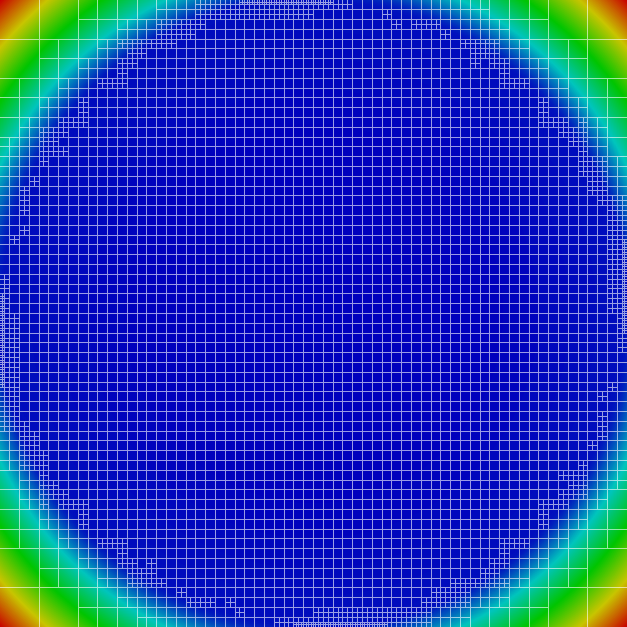
\includegraphics[width=1.0\textwidth]{Vortex/modified6nc.png}

Nonconservative
\end{figure}
\end{column}
\begin{column}{0.49\textwidth}
\begin{figure}
\centering
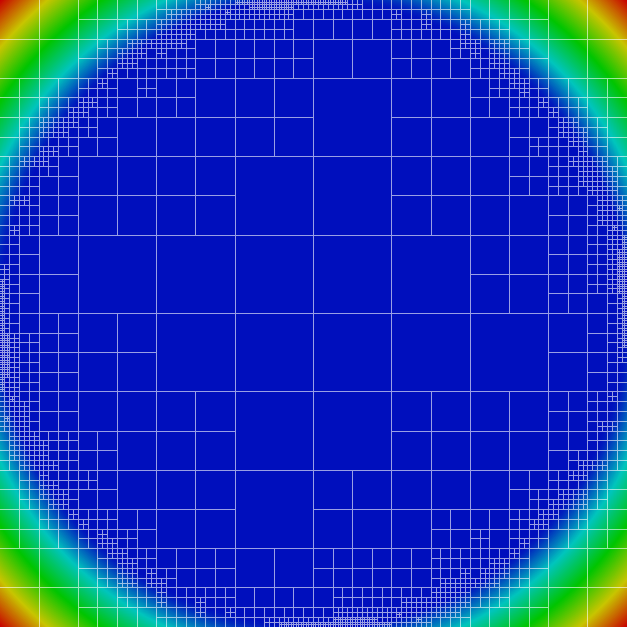
\includegraphics[width=1.0\textwidth]{Vortex/modified6c.png}

Conservative
\end{figure}
\end{column}
\end{columns}
}
\only<2>{
\begin{figure}[t]
\centering
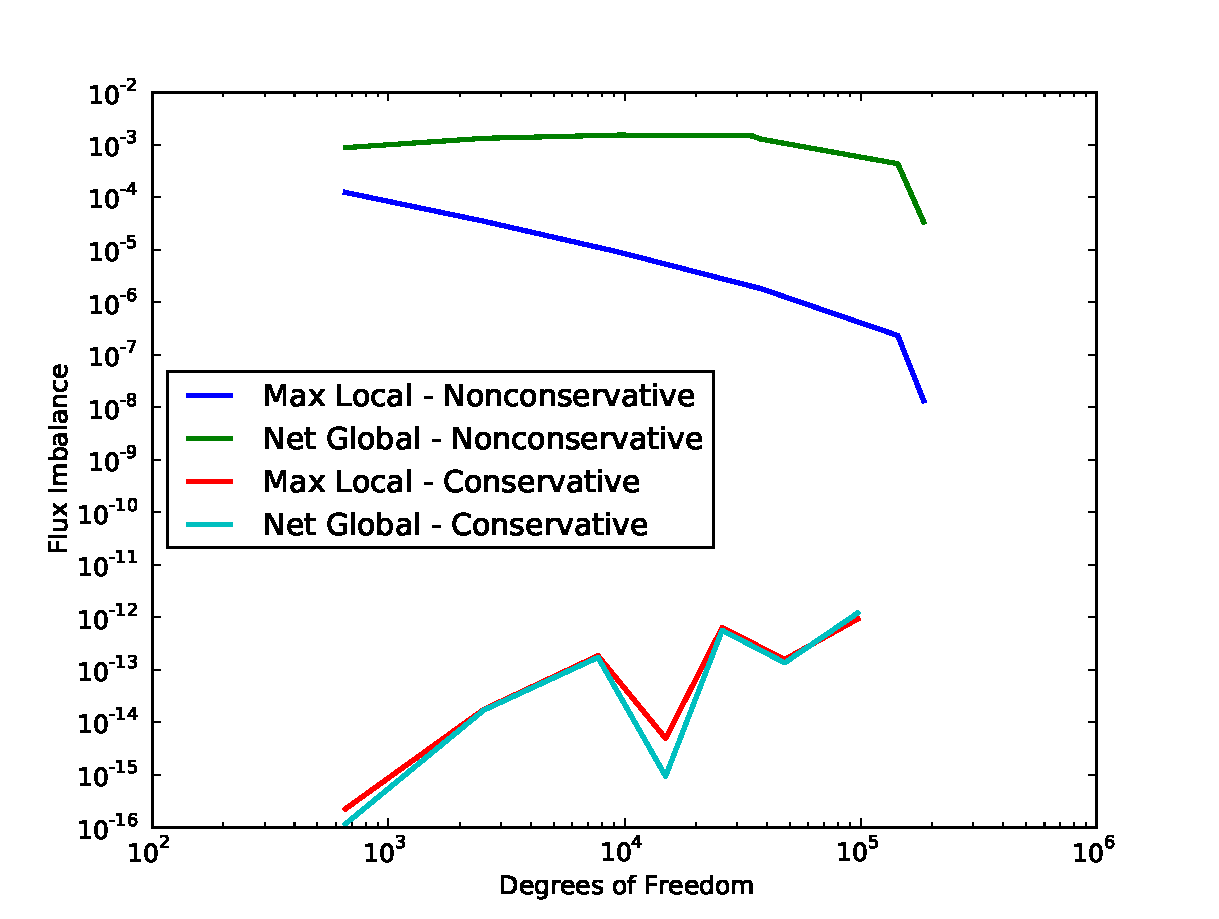
\includegraphics[width=0.7\textwidth]{Vortex/modifiedFlux.pdf}
\end{figure}
}
\end{frame}
\begin{comment}
\end{comment}


%===============================================================================
% NEW SLIDE
%===============================================================================
\begin{frame}
\frametitle{Discontinuous Source Problem}
After 8 refinements, $\epsilon=10^{-3}$,
$\bfbeta=(0.5,1)^T/\sqrt{1.25}$, $\hat g=
\begin{cases}
1, & y >=2x\\
0, & y <2x
\end{cases}$
\only<1>{
\begin{columns}
\begin{column}{0.49\textwidth}
\begin{figure}
\centering
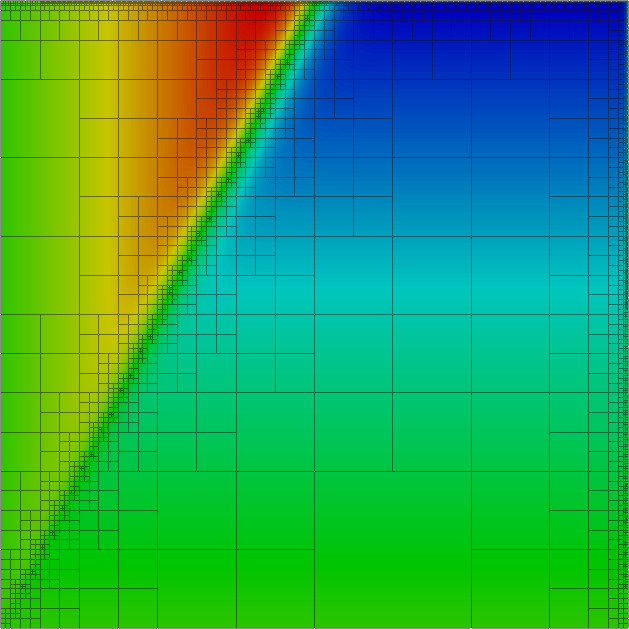
\includegraphics[width=1.0\textwidth]{Discontinuous/modified8nc.png}

Nonconservative
\end{figure}
\end{column}
\begin{column}{0.49\textwidth}
\begin{figure}
\centering
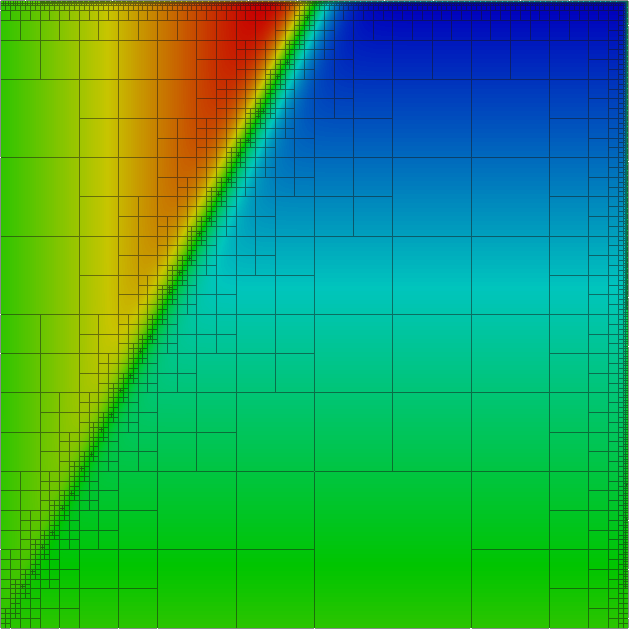
\includegraphics[width=1.0\textwidth]{Discontinuous/modified8c.png}

Conservative
\end{figure}
\end{column}
\end{columns}
}
\only<2>{
\begin{figure}[t]
\centering
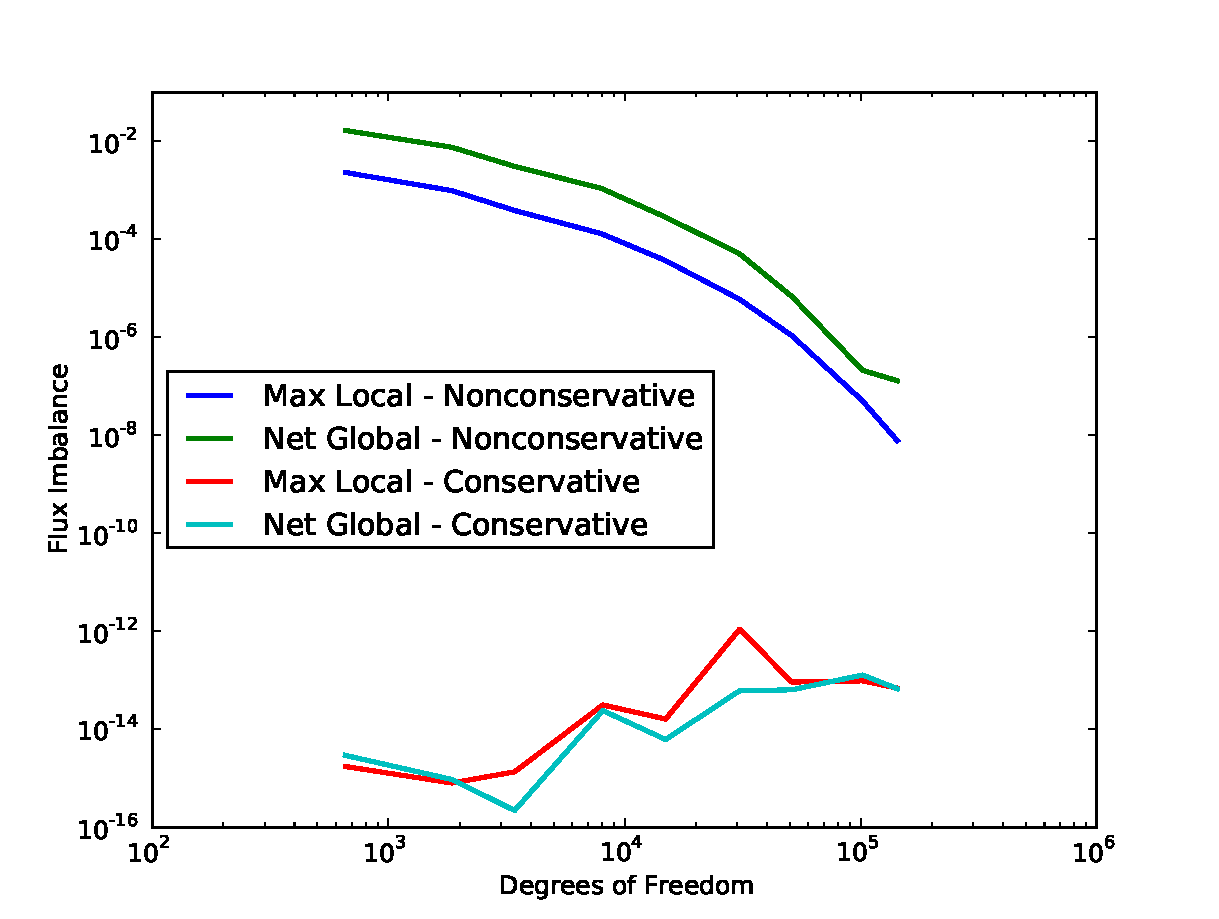
\includegraphics[width=0.7\textwidth]{Discontinuous/modifiedFlux.pdf}
\end{figure}
}
\end{frame}
\begin{comment}
\end{comment}


%===============================================================================
% NEW SLIDE
%===============================================================================
\begin{frame}
\frametitle{Inviscid Burgers' Equation}
\only<1>{
\vspace{-0.5em}
\[
\frac{\partial u}{\partial t}+u\frac{\partial u}{\partial
x}=0
\quad\Leftrightarrow\quad
\nabla_{x,t}\cdot\left(\begin{array}{c}
\frac{u^2}{2}\\
u
\end{array}\right)=0
\]
\vspace{-1.5em}
\begin{columns}
\begin{column}{0.49\textwidth}
\begin{figure}
\centering
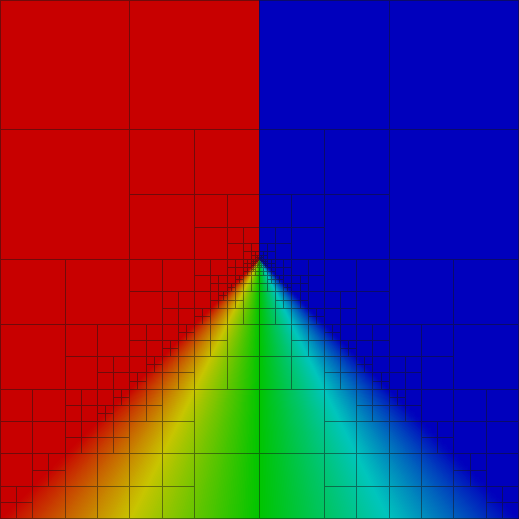
\includegraphics[width=1.0\textwidth]{Burgers/graph8nc.png}

Nonconservative
\end{figure}
\end{column}
\begin{column}{0.49\textwidth}
\begin{figure}
\centering
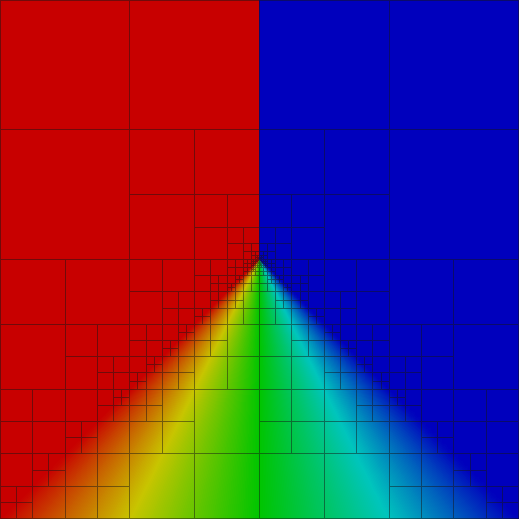
\includegraphics[width=1.0\textwidth]{Burgers/graph8c.png}

Conservative
\end{figure}
\end{column}
\end{columns}
}
\only<2>{
\begin{figure}[t]
\centering
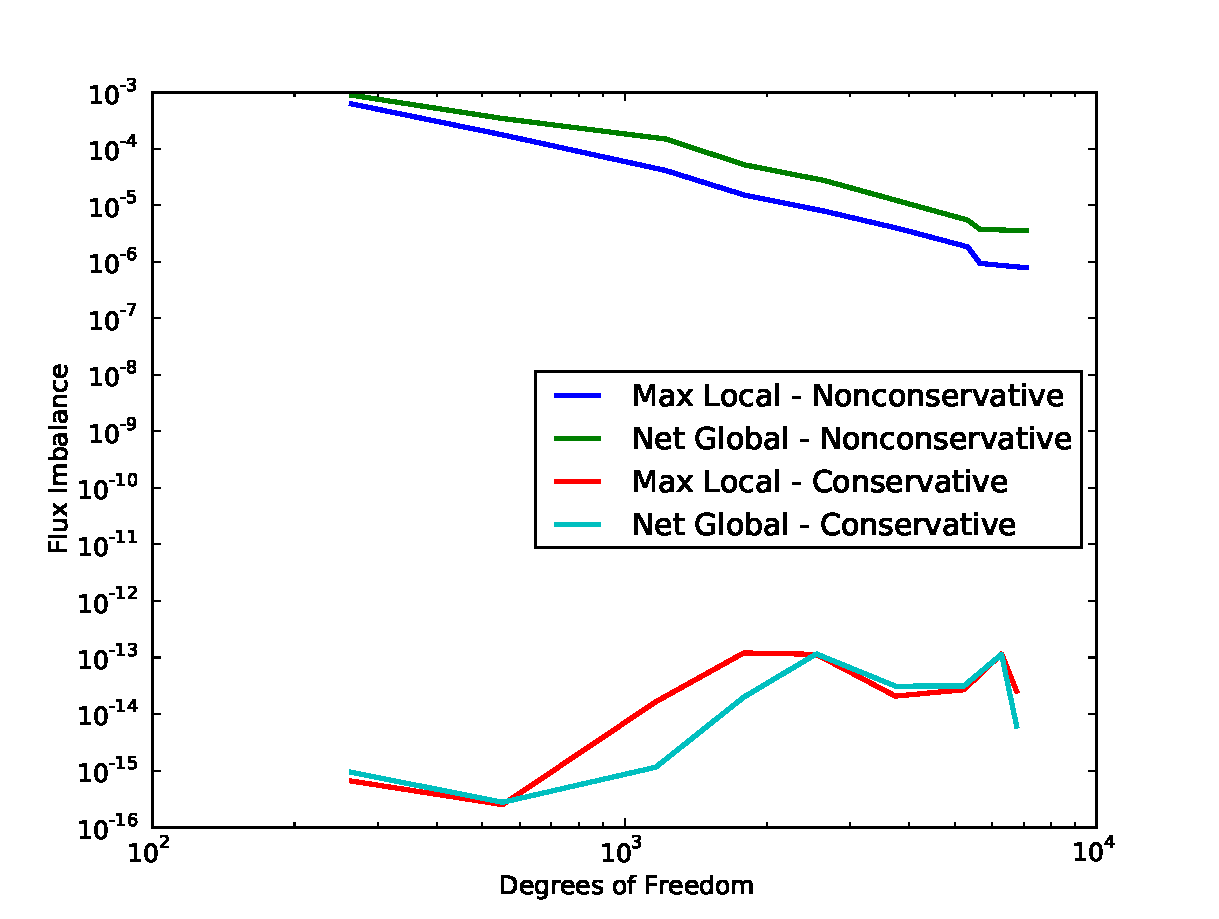
\includegraphics[width=0.7\textwidth]{Burgers/graphFlux.pdf}
\end{figure}
}
\end{frame}
\begin{comment}
This problem is slightly off-topic in that we are no longer dealing with the
convection-diffusion equation. Instead we consider the inviscid Burgers
equation which can be formulated as a nonlinear hyperbolic conservation law,
letting us relate directly to the Lax-Wendroff theorem. A common argument for
local conservation is that shock speed can be off if we don't have a
conservative method, and the Burgers' equation is often given as an example.
We choose to work with a space-time formulation where x follows the x axis and
time the y. So without going through the DPG derivation, let's just see how
our two methods behave. Apart from some slight differences in refinement
pattern, the two methods appear nearly identical.
\end{comment}


%===============================================================================
% NEW SLIDE
%===============================================================================
\begin{frame}
\frametitle{Stokes Flow Around a Cylinder}
\begin{columns}
\begin{column}{0.49\textwidth}
\only<1>{
\begin{figure}
\centering
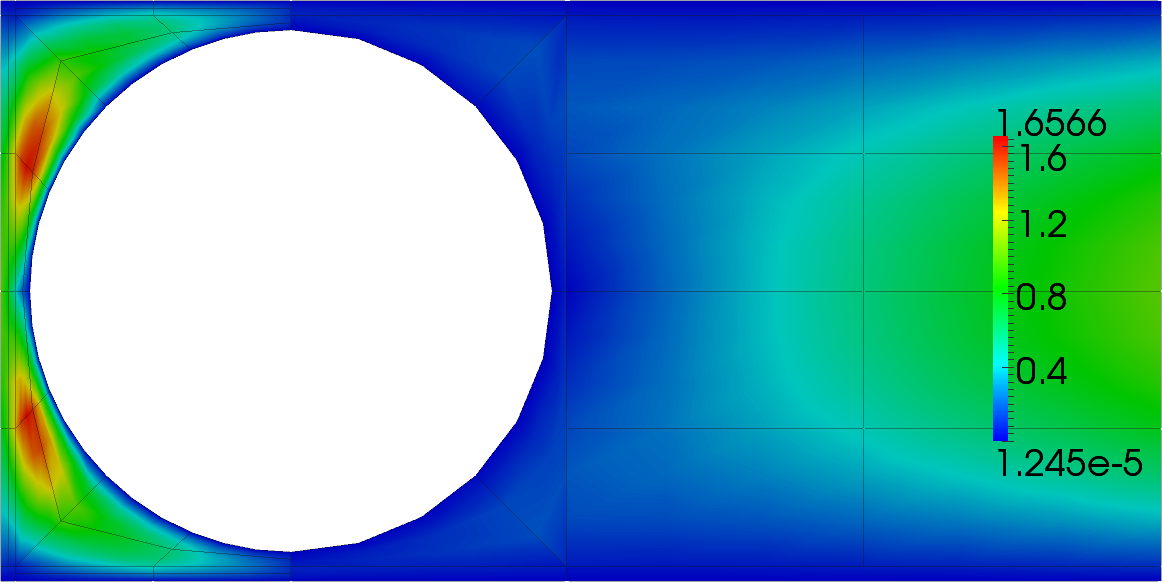
\includegraphics[width=1.0\textwidth]{StokesCylinder/umag9_NC1.png}\\
\vspace{-1ex}
{\scriptsize 1 Refinement}\\
\vspace{1ex}
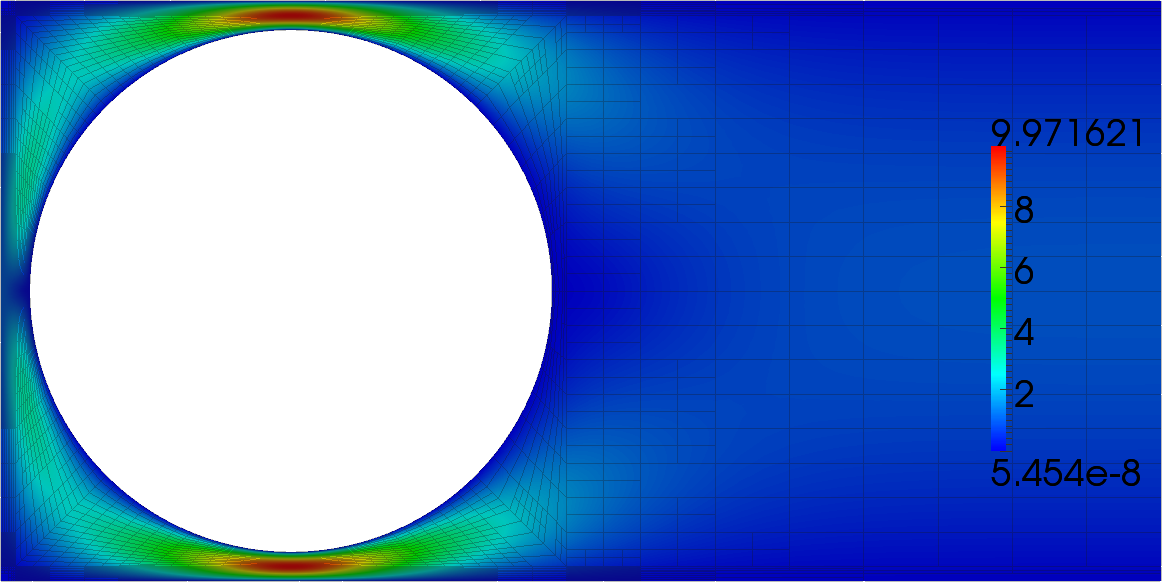
\includegraphics[width=1.0\textwidth]{StokesCylinder/umag9_NC6.png}
\vspace{-1ex}
{\scriptsize 6 Refinements}
\vspace{1ex}

Nonconservative
\end{figure}
\end{column}
\begin{column}{0.49\textwidth}
\begin{figure}
\centering
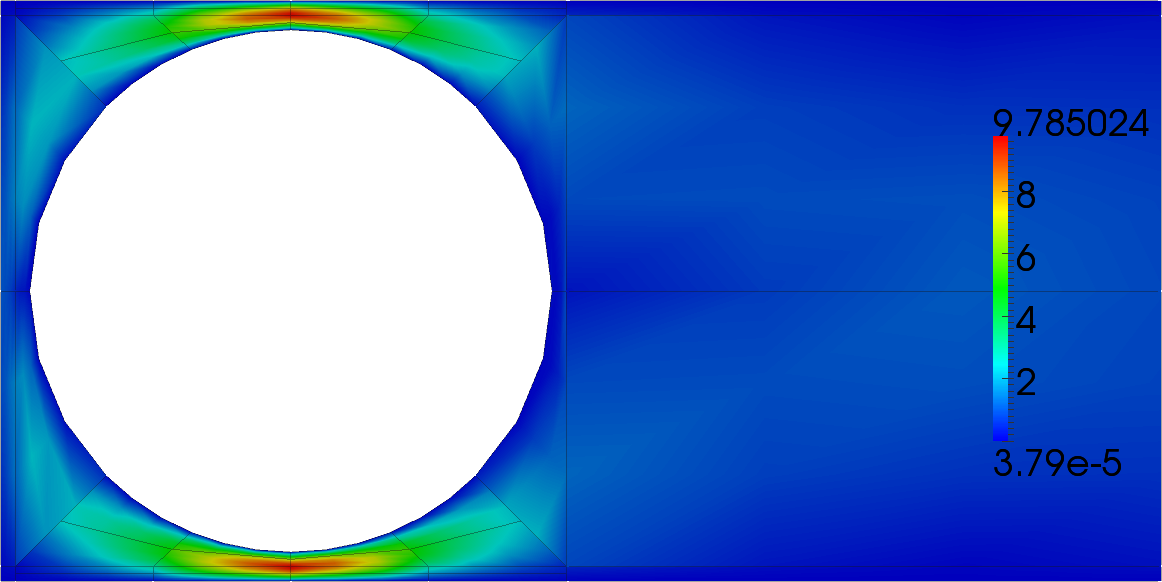
\includegraphics[width=1.0\textwidth]{StokesCylinder/umag9_C1.png}\\
\vspace{-1ex}
{\scriptsize 1 Refinement}\\
\vspace{1ex}
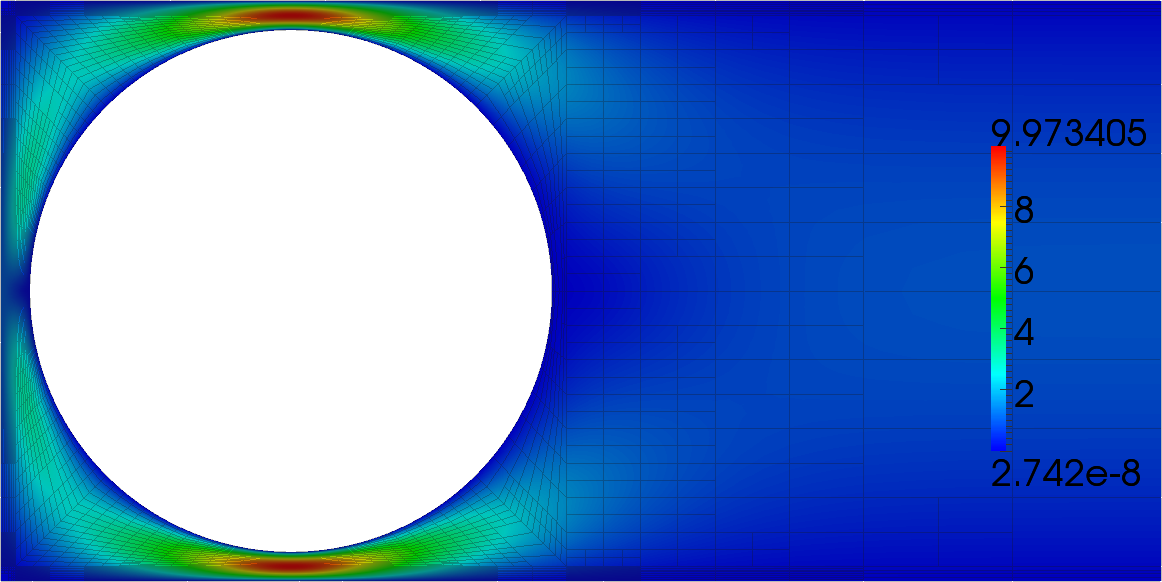
\includegraphics[width=1.0\textwidth]{StokesCylinder/umag9_C6.png}
\vspace{-1ex}
{\scriptsize 6 Refinements}
\vspace{1ex}

Conservative
\end{figure}
}
\only<2>{
\begin{figure}[t]
\centering
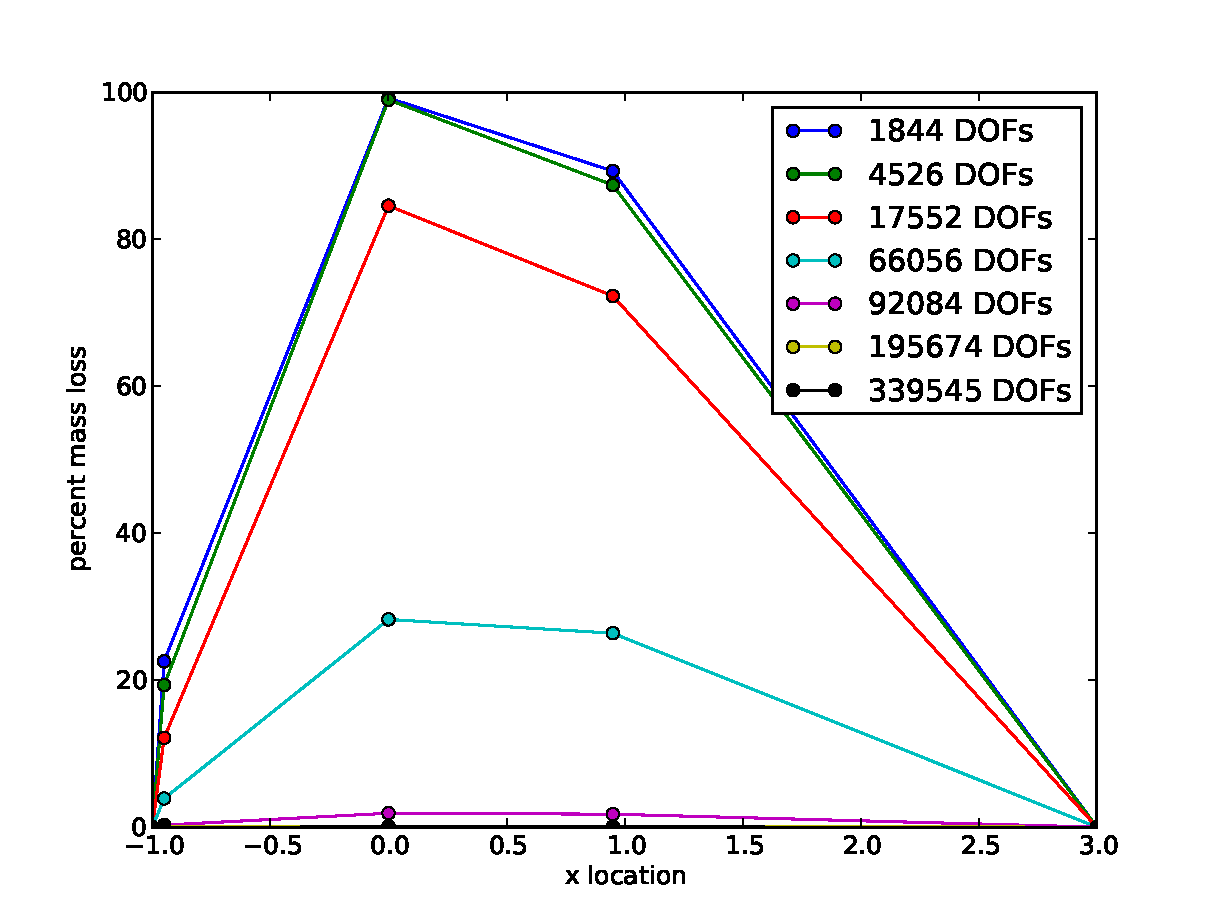
\includegraphics[width=1.1\textwidth]{StokesCylinder/MassLoss9_NC.pdf}

Nonconservative
\end{figure}
\end{column}
\begin{column}{0.49\textwidth}
\begin{figure}[t]
\centering
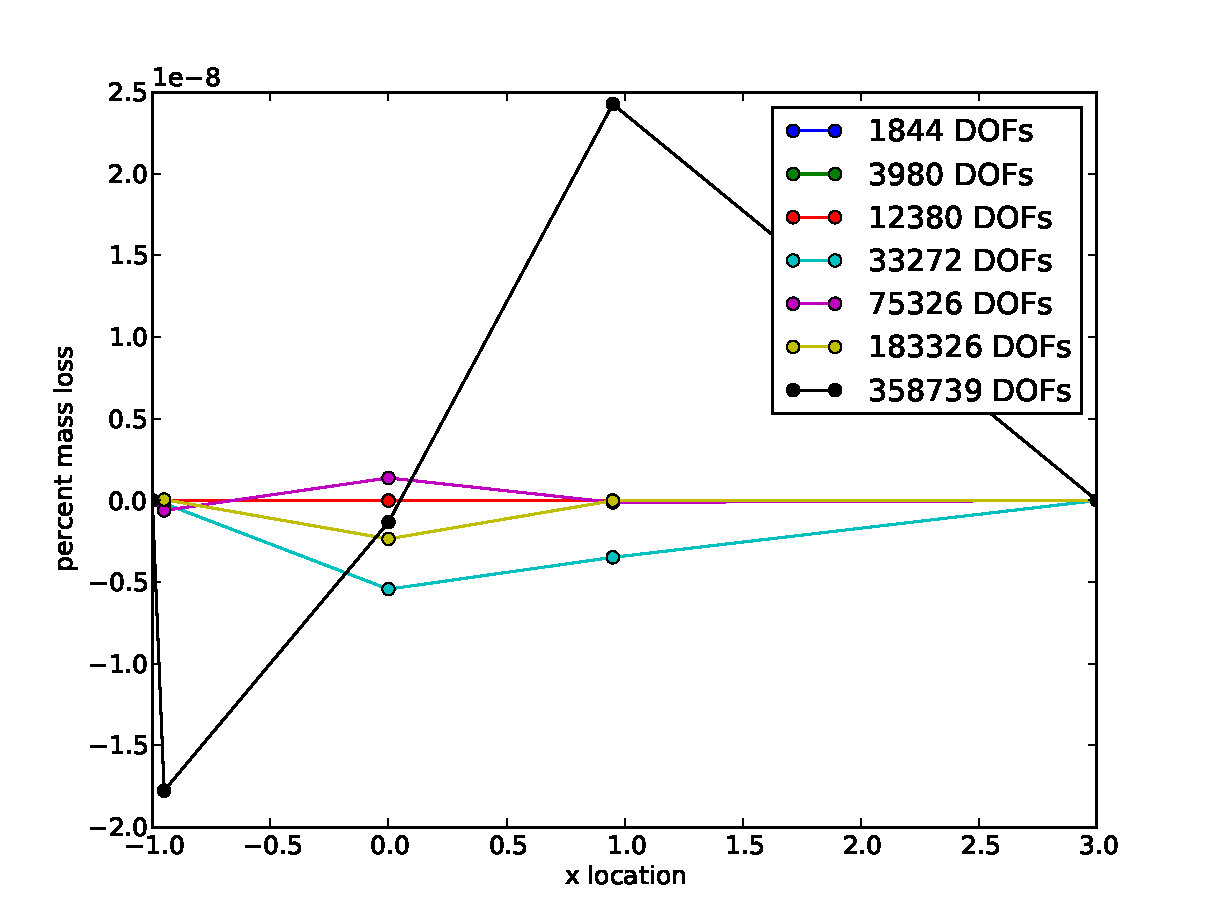
\includegraphics[width=1.1\textwidth]{StokesCylinder/MassLoss9_C.pdf}

Conservative
\end{figure}
}
\end{column}
\end{columns}
\end{frame}
\begin{comment}
\end{comment}


%===============================================================================
% NEW SLIDE
%===============================================================================
\begin{frame}
\frametitle{Stokes Flow Backward Facing Step}
\begin{columns}
\begin{column}{0.49\textwidth}
\only<1>{
\begin{figure}
\centering
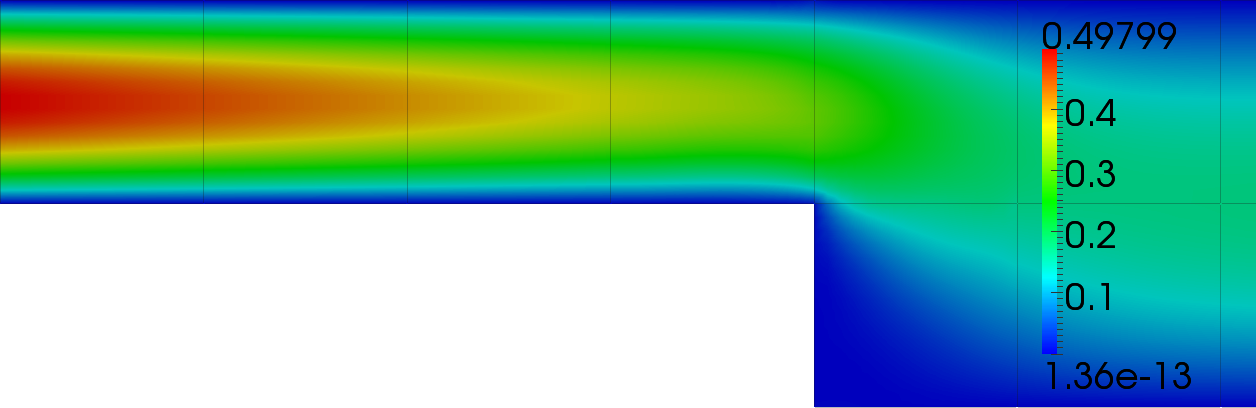
\includegraphics[width=1.0\textwidth]{StokesStep/Quartic_NC0.png}\\
\vspace{-1ex}
{\scriptsize Initial Mesh}\\
\vspace{1ex}
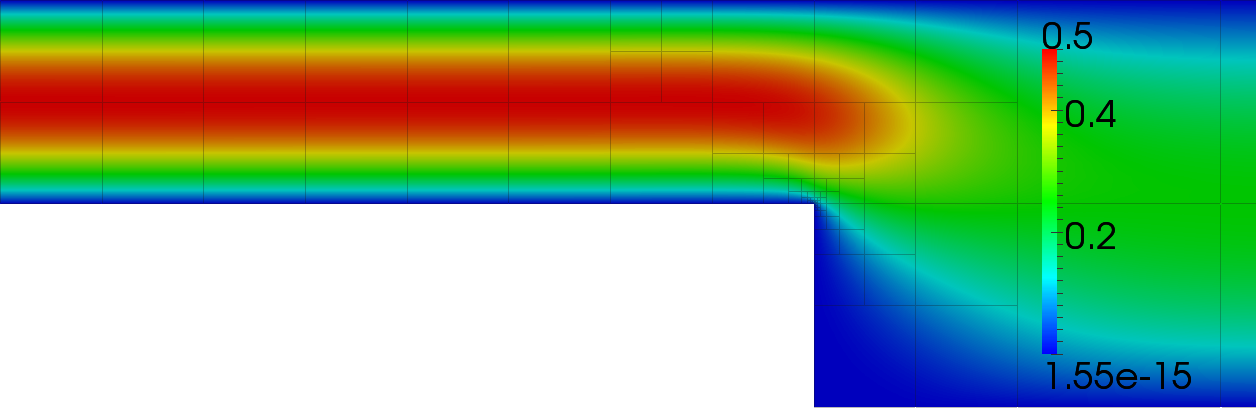
\includegraphics[width=1.0\textwidth]{StokesStep/Quartic_NC8.png}
\vspace{-1ex}
{\scriptsize 8 Refinements}
\vspace{1ex}

Nonconservative
\end{figure}
\end{column}
\begin{column}{0.49\textwidth}
\begin{figure}
\centering
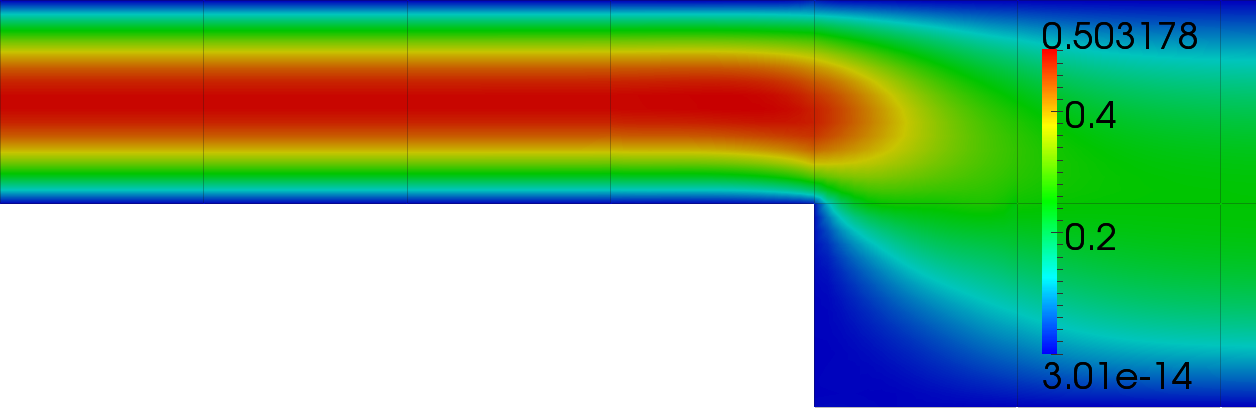
\includegraphics[width=1.0\textwidth]{StokesStep/Quartic_C0.png}\\
\vspace{-1ex}
{\scriptsize Initial Mesh}\\
\vspace{1ex}
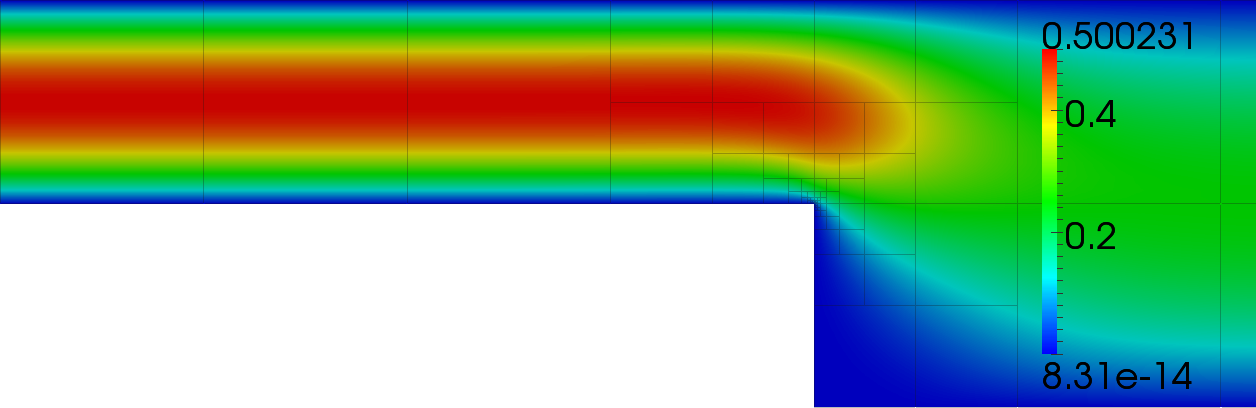
\includegraphics[width=1.0\textwidth]{StokesStep/Quartic_C8.png}
\vspace{-1ex}
{\scriptsize 8 Refinements}
\vspace{1ex}

Conservative
\end{figure}
}
\only<2>{
\begin{figure}[t]
\centering
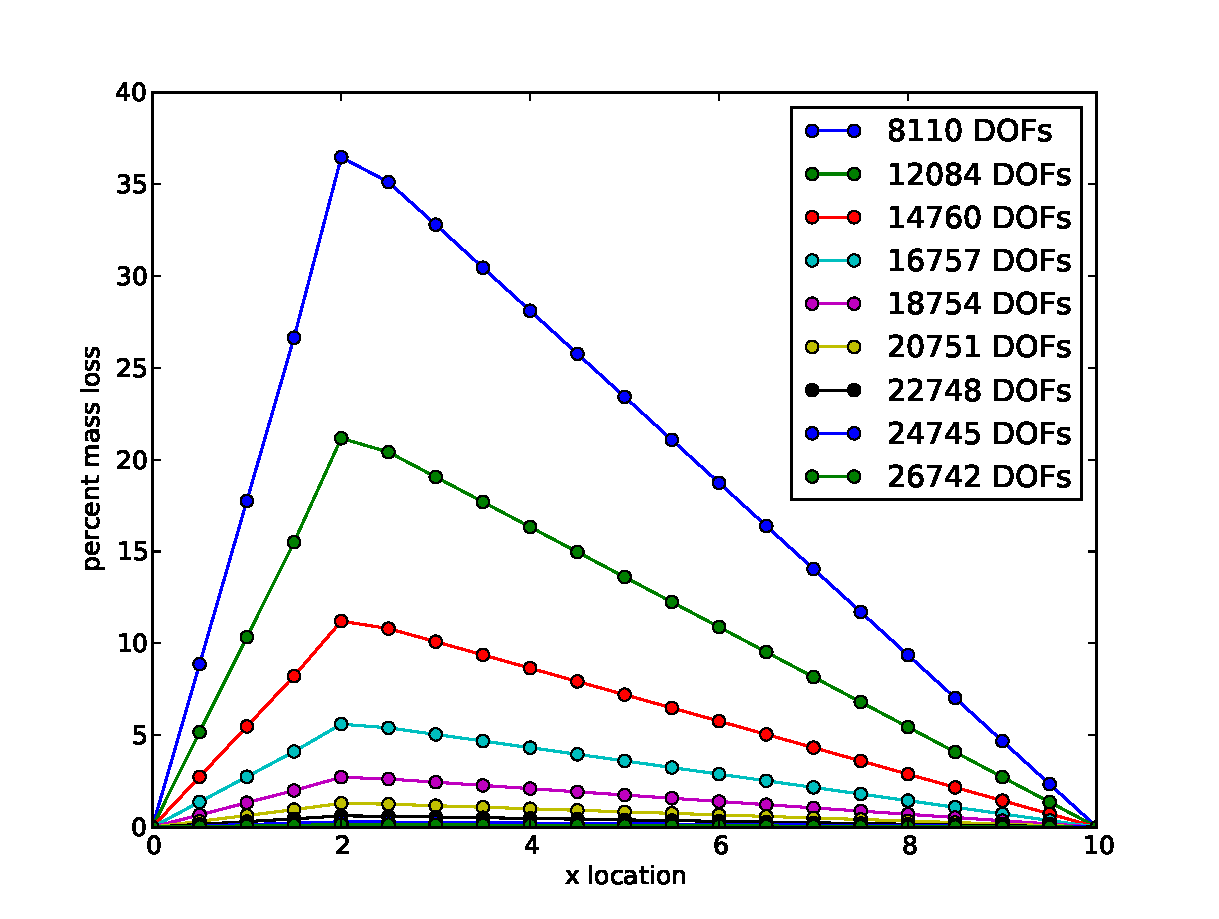
\includegraphics[width=1.1\textwidth]{StokesStep/MassLoss_NC.pdf}

Nonconservative
\end{figure}
\end{column}
\begin{column}{0.49\textwidth}
\begin{figure}[t]
\centering
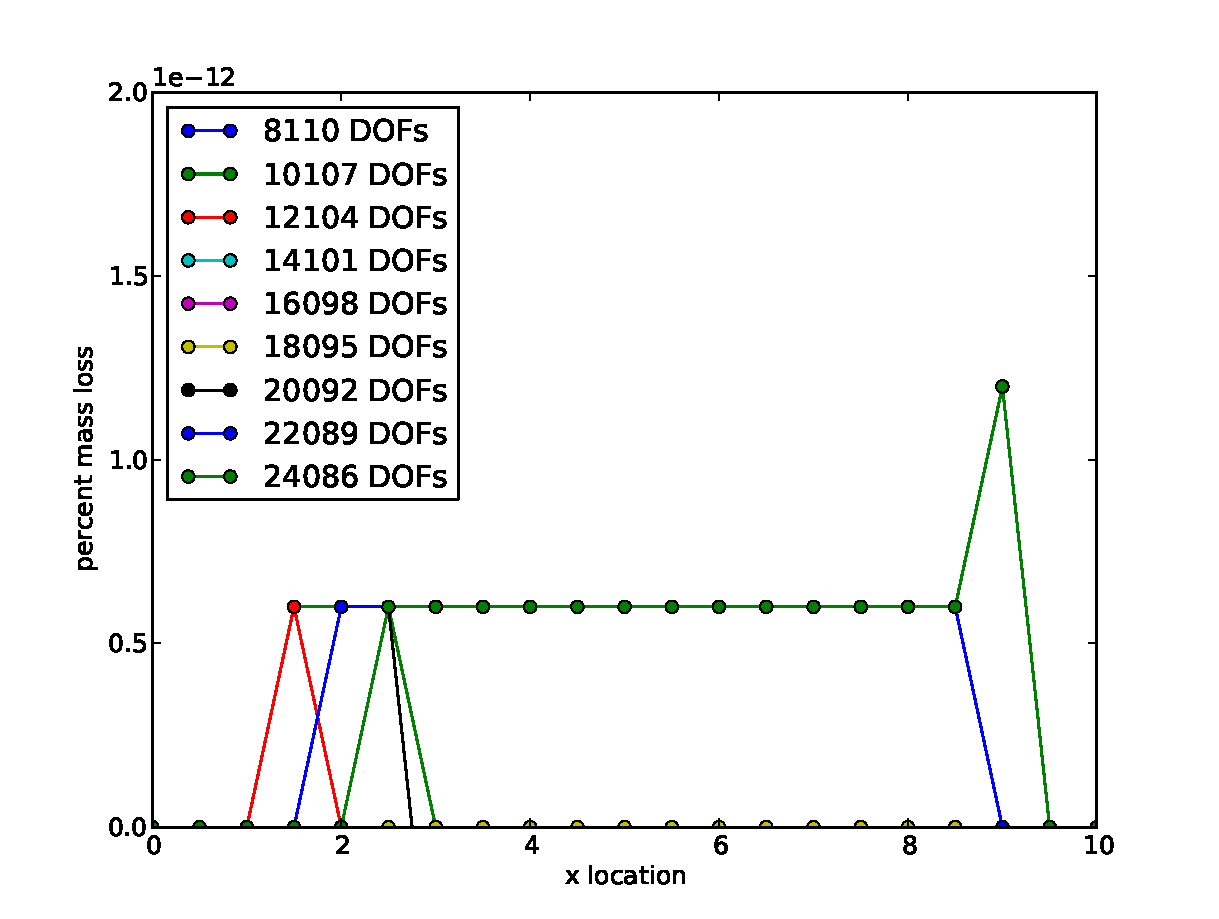
\includegraphics[width=1.1\textwidth]{StokesStep/MassLoss_C.pdf}

Conservative
\end{figure}
}
\end{column}
\end{columns}
\end{frame}
\begin{comment}
\end{comment}


%===============================================================================
% NEW SLIDE
%===============================================================================
\begin{frame}
\frametitle{Summary}
What have we done?
\begin{itemize}
\item We've turned our minimization problem into a saddlepoint problem.
\item The change is computationally feasible.
\item Mathematically, it gets rid of troublesome term.
\end{itemize}

\vspace{2ex}
Does it make a difference?
\begin{itemize}
\item Enforcement changes refinement strategy.
\item Some improvement on condition number for local solves.
\item Standard DPG is nearly conservative for many of the problems considered,
  but seems to suffer from mass loss similar to other LSFEM methods.
\item For some problems, local conservation allows us to converge to a
  reasonable solution on a much coarser mesh.
\end{itemize}
% \vspace{2ex}
% \visible<2->{\pecosbold{We need to study the effect on real fluid dynamics.}}
\end{frame}


\bibliographystyle{plain}
{\scriptsize
\bibliography{../DPG.bib}
}

\end{document}
